\documentclass[journal, compsoc]{IEEEtran}

\usepackage{graphicx}
\usepackage{algorithm}
\usepackage{algpseudocode}
\usepackage{amsmath}
\usepackage{amsfonts}
\usepackage{hyperref}
\usepackage{mathtools}

\newcommand\Mycomb[2][^n]{\prescript{#1\mkern-0.5mu}{}C_{#2}}

\title{Artificial Intelligence Report on Solutions to Laboratory Problems}

\author{Siddhartha~Tiwari, Siddharth~Mani~Tiwari, Saurabh~Kumar, Pushkar~Tiwari}

%\author{
%\IEEEauthorblockN{Siddhartha Tiwari}\IEEEauthorblockA{201851127}
%\and
%\IEEEauthorblockN{Siddharth Mani Tiwari}\IEEEauthorblockA{201851126}
%\and
%\IEEEauthorblockN{Saurabh Kumar}\IEEEauthorblockA{201851113}
%\and
%\IEEEauthorblockN{Pushkar Tiwari}\IEEEauthorblockA{201851095}
%}

\begin{document}
\IEEEtitleabstractindextext{%
\begin{abstract}
This report discusses and solves various laboratory problems assigned to us by Dr. Pratik Shah. The problems discussed are from various fields including State Space Search, Heauristics based search, Simulated Annealing, Alpha-Beta Pruning, Causal Bayesian Networks. For each problem, the most efficient solution is arrived upon gradually, using different techniques taught in the class.
\end{abstract}
}
\maketitle
\section{The Rabbit Leap Problem}
\subsection{Introduction}

In the rabbit leap problem, $3$ rabbits right-bound rabbits stand in a line blocked by $3$ left-bound rabbits with a empty stone between them.
The rabbits can only move forward one step or two steps. They can jump over one rabbit if the need arises, but not more than that. 
The problem is to find a sequence of rabbit jumps such that all the rabbits are in the direction they intended to go to.

\subsection{Modelling}

The problem can be modeled as a state search problem. Consider the start state. Assume that the left bound frogs are represented by
the letter $L$ and the right bound frogs are represented by the letter $R$. The empty stone can be represented by a underscore(\_).
So, each state can now be represented as a string of exactly seven characters. For example, the string representation of the start state is \textbf{LLL\_RRR}.

Given this representation, the state space consists of all such states reachable by the start state by using some number of moves,
according to the problem statement. Each transition from one state to the other is equivalent to one valid move.
So, the state transition diagram looks like in figure \ref{fig_sim}.

\begin{figure}[!h]
\centering
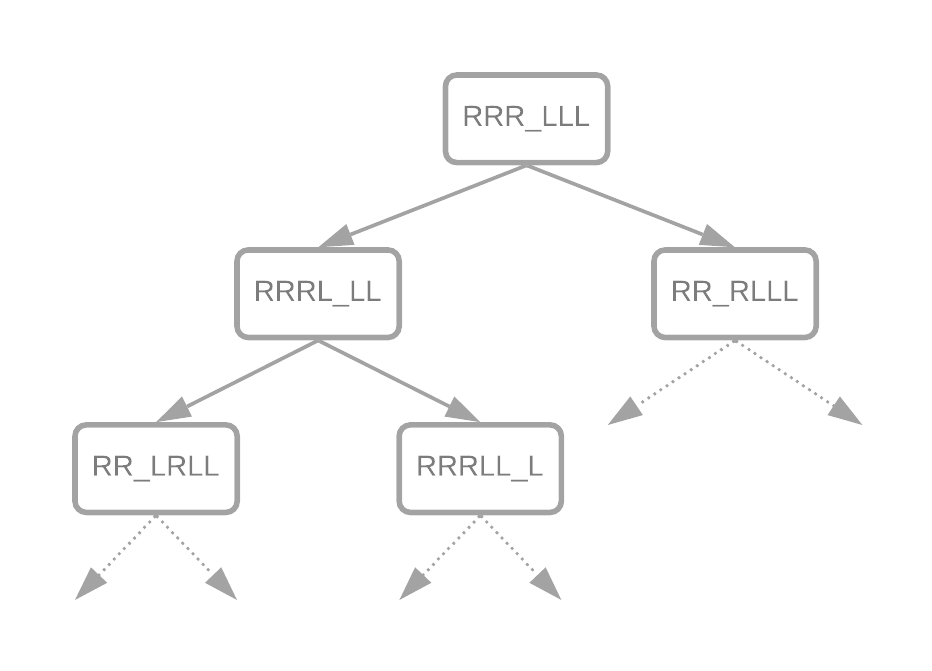
\includegraphics[width=2.5in]{rabbitleap.png}
\caption{State Space of the Rabbit Leap problem}
\label{fig_sim}
\end{figure}

Thus, the Rabbit Leap problem is just an instance of the state space search. The state space along with the moves can be thought of as a graph,
where each edge is a move.

\subsection{Size of the state space search}

The state space of the Rabbit Leap problem, contains all the states reachable by start state, using some number of moves.
One important thing to note is that, for any two states $u$ and $v$, there is at most one directed path that connects $u$ and $v$.
This is because, the movement of the rabbits can only be in one direction (left for left-bound rabbits and right for right-bound rabbits).
Thus, the state space graph is a tree (acyclic connected graph).

Now, since the $7$ letters used in the string to represent a state can vary by a total of $\frac{7!}{3!3!} = 140$, the upper bound on the size of the state space is thus $140$.
Note the actual number of states the search algorithms described later, are going to explore might be much less than $140$.

\subsection{Breadth First Search Solution}

The Breadth first search solution, first explores all the states that are at the same depth in the state space tree,
and then explores all the states of the next depth and so on.
Here is an algorithm that represents the Depth First Solution to this problem.

\begin{algorithm}
\caption{Breadth First Search}\label{BFSrabbit}
\begin{algorithmic}[1]
\Procedure{BFS}{$s,g, start$}\Comment{the state graph, the goal and start state}
\State $visited \gets \{\}$
\State $frontier \gets \{start\}$ \Comment{frontier is a queue.}
\While{$frontier.size$ $\neq$ 0}
\State $curr \gets frontier.dequeue()$
\If{$curr = gl$}
\State \textbf{return} $start \rightarrow curr$
\EndIf
\State $frontier.enqueue(curr.children \notin visited)$
\State $visited \gets visited + \{curr\}$
\EndWhile\label{bfsendwhile}
\EndProcedure
\end{algorithmic}
\end{algorithm}

Now, since BFS first visits all the states at depth, say $d$, in the state tree, whenever it gets a solution
we can say that this solution is $d$ moves away from the starting state and that no other solution exist with less than $d$
moves (because then BFS would get the solution at less than $d$ depth only). \textbf{So, the solution obtained by BFS is the optimal one}.

\subsection{Depth First Search Solution}

The DFS solution, first explores all the nodes of a branch with increasing depths, and then backtrack to choose a different
branch to explore. The algorithm of Depth First Search is given below.

\begin{algorithm}
\caption{Depth First Search}\label{BFSrabbit}
\begin{algorithmic}[1]
\Procedure{DFS}{$s,g, start$}\Comment{the state graph, the goal and start state}
\State $visited \gets \{\}$
\State $frontier \gets \{start\}$ \Comment{frontier is a stack.}
\While{$frontier.size$ $\neq$ 0}
\State $curr \gets frontier.pop()$
\If{$curr = gl$}
\State \textbf{return} $start \rightarrow curr$
\EndIf
\State $frontier.push(curr.children \notin visited)$
\State $visited \gets visited + \{curr\}$
\EndWhile\label{bfsendwhile}
\EndProcedure
\end{algorithmic}
\end{algorithm}

As it is evident from the algorithm above, there is very little difference between DFS and BFS solutions. In BFS we have
chosen a queue to store the frontier states, while in DFS a stack is used. Thus, in stack whenever a node is added it is going
to be explored immediately. This enforces the Depth First Search.

\section{Challenge Problem: Jigsaw Puzzle}
\subsection{Introduction}

The problem is pretty clear. We have to design an intelligent agent to solve a jigsaw puzzle. The first assumption we are taking is, that
every input image will have a resolution of $512 \times 512$. The second assumption, is that the total number of blocks in the jigsaw is
exactly $9$ and each block is a square. We will take an image, initially unscrambled, scramble it and then try to solve it with our agent.
The programming language we are going to use is MATLAB\textsuperscript{$\copyright$}.

\subsection{Discussion of solution}

The problem is not straightforward to solve. In this problem, the goal state is not defined (we can identify the goal state, but the
computers cannot). Hence this problem is a classic example of Simulated Annealing. In Simulated Annealing, we define the entropy of each
state and the objective is to minimize the entropy using probabilistic jumps. Assume that this entropy of any state $s$ is defined as:
\[
    E(s), \text{ where} \min{(E(s))} = E(goal)
\]

At any moment of time, simulated annealing picks up any two blocks of the image. Assume that the initial state is $i$ and the state
obtained after swapping these two blocks is $f$. Then simulated annealing does the following:

\[
     \begin{cases}
       \text{swap,} &\quad\text{if } E(f) < E(i)\\
       \text{swap,} &\quad\text{with a probability of } e^{\frac{E(i) - E(f)}{c}} \text{ if } E(f) > E(i)\\
       \text{do nothing,} &\quad\text{otherwise}\\
     \end{cases}
\]

Now, solving this problem depends on whether there is such Entropy function or not. This is exlored in the next section.

\subsection{The Entropy function}

As soon as we scramble an image, we are disturbing the smoothness of that image. This roughness occurs at the common edges of the square
blocks. The more the square blocks are not in their position, the more the roughness is going to be. The way to measure this roughness,
mathematically, is to find out how sudden is the change in the values of the pixels occuring. The gradient of a function exactly represents this
quantity.

To verify whether this works or not, we tried different gradient plots for different scrambled states of the images, and the table \ref{tab:grad}
shows the total gradient of different states compared to the total gradient of the original state.

\begin{table}[!h]
\renewcommand{\arraystretch}{1.3}
\caption{Gradient Variations}
\label{tab:grad}
\centering
\begin{tabular}{c||c||c}
\hline
\bfseries No of blocks out of position & \bfseries Total Gradient & \bfseries \% increase\\
\hline\hline
0 & 1824165.5 & 0.00\\
3 & 1840341.5 & 0.89\\
6 & 1876673.5 & 2.88\\
7 & 1885794.0 & 3.38\\
10 & 1.9294755 & 5.77\\
\hline
\end{tabular}
\end{table}

The surface plots of the gradients of original image and a scrambled image is given in figure \ref{img:scr}.

\begin{figure}[!h]
\label{img:scr}
\minipage{0.5\linewidth}
  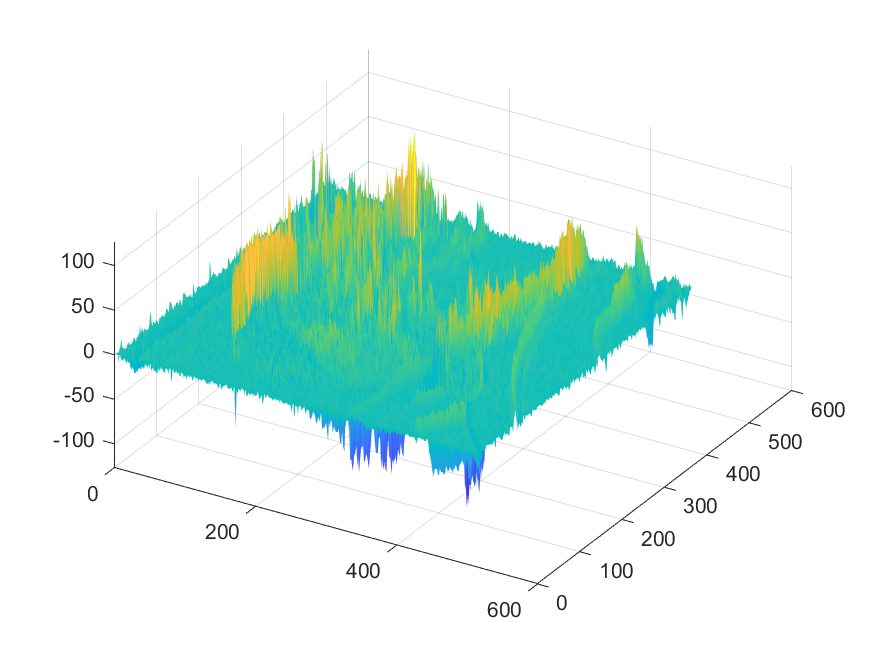
\includegraphics[width=\linewidth]{less_scrambled_gradient.pdf}
  \caption{Original Image}
\endminipage\hfill
\minipage{0.5\linewidth}
  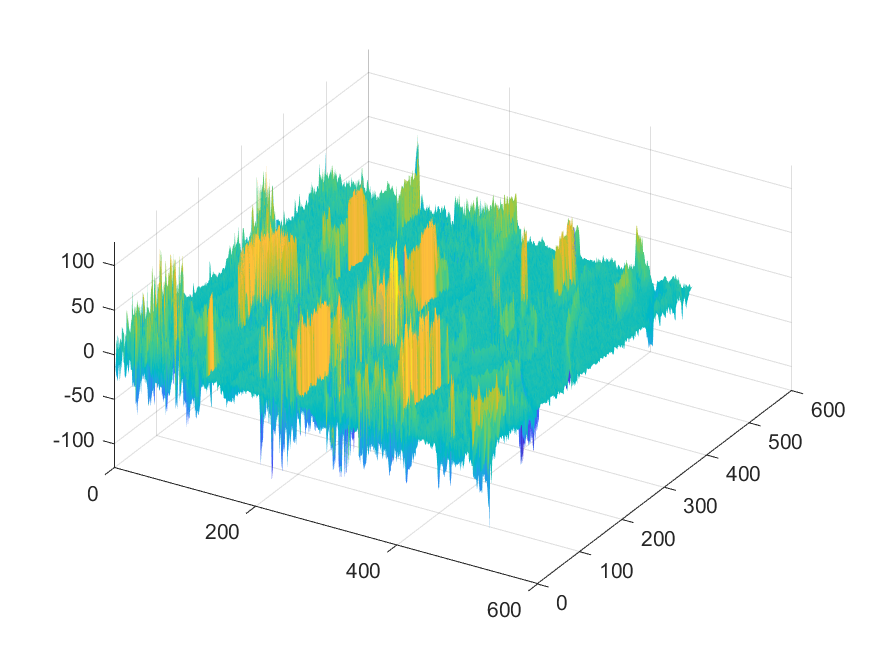
\includegraphics[width=\linewidth]{scrambled_gradient.pdf}
  \caption{Scrambled Image}
\endminipage
\end{figure}

It is evident from the picture that the scrambled image has a higher gradient than the original image.
So, we can say that the roughness increases as the number of blocks out of position in the image increases.

Thus, after a lot of exploration, we can say that the absolute sum of gradients of the pixel array of any image can act
as the Entropy for Simulated Annealing. The entropy function can be written as in equation \ref{eq:entr}.
\begin{equation}
E(I(x,y)) = \sum_{x,y} |\nabla I(x,y)|
\label{eq:entr}
\end{equation}

\subsection{Implementation}

The implementation of the simulated annealing is given in Algorithm \ref{algo:sim}. The matlab live code file can be found at the link
provided above.

\begin{algorithm}
\caption{Simulated Annealing}\label{algo:sim}
\begin{algorithmic}[1]
\Procedure{Simulated Annealing}{$img$}\Comment{img is the $2-$D array of pixels of the image.}
\State $iterations \gets 100$
\State $it \gets 0$
\State $i \gets img$ \Comment{Start state is the original image.}
\State $C \gets 1000$
\While{$it \neq iterations$}
\State $f \gets $ rand\_swap\_block() \Comment{random swapping}
\If{$E(f) \leq E(i)$}
\State $i \gets f$
\ElsIf{$rand(0, 1) \leq e^{\frac{(E(i) - E(f))}{C}}$}
\State $i \gets f$
\EndIf
\State $it \gets it + 1$
\EndWhile
\State \textbf{return } $i$
\EndProcedure
\end{algorithmic}
\end{algorithm}

\subsection{Other Solutions}
After running the algorithm a number of times we came to the conclusion that this form of simulated annealing does not solve the problem
completely. So, we tried a different entropy function for the edge detection. It takes two square blocks of the picture and find the average
values of pixel along the common edge. Thus, we find all such possible combinations of two edges. After that, we assigned a cost to each
such edge using the difference between the average values calculated. Now, to do simulated annealing the entropy of a state is the total cost
of all the edges of the picture.\\
We also tried various other sub-algorithms like grouping 4 picture blocks into one if the total cost of all the edges in the block is close
to zero. All these solutions we tried is in the Jigsaw folder of our repository. Here is the \href{https://github.com/sid-tiw/AI-codes/tree/main/codes/Jigsaw}{link} to the folder.

\section{Travelling Salesman Problem}
\subsection{Introduction}
The objective of this problem is to find the most optimal hamiltonian cycle. A hamiltonian cycle is a loop that visits each of the
vertices of a graph exactly once, except the first and the last vertex. The problem is used in multiple practical purposes. One is
to find out the most optimal path visiting a given set of cities with least travel as possible.

\subsection{Solution}
We are using Simulated annealing to solve this problem sub-optimally. We used test cases from \cite{test_case} to test the program.
We used two ideas to update the Hamiltonian cycle in a given iteration. The first idea is to choose a subpath of the hamiltonian cycle
and then replace it with the reverse of the subpath. The another is that instead of replacing the reverse of the subpath, permute the
subpath with a random premutation, and then replace it in the hamiltonian cycle.\\
The two approaches surprisingly differ by a much margin. The results of these two approaches is given in the table below.
\begin{table}[!h]
\renewcommand{\arraystretch}{0.4}
\caption{Reversing the subpath}
\label{tab:cost}
\centering
\begin{tabular}{c||c||c||c}
\hline
\bfseries No of points & \bfseries reversing & permuting & \bfseries actual path cost\\
\hline\hline
131 & 601 & 2380 & 564\\
237 & 1530 & 4132 & 1019\\
380 & 1911 & 7012 & 1621\\
423 & 1810 & 9000 & 1365\\
662 & 4815 & 12000 & 2513\\
\hline
\end{tabular}
\end{table}


Clearly, the algorithm performs better when the subpath is reversed compared to when it is permuted. We tried but failed to find the
exact reason behind this.\\
We chose $20$ tourist locations of Rajashtan to find the sub-optimal path connecting all the cities. The result is in the live code
file at \href{https://github.com/sid-tiw/AI-codes/blob/main/codes/Traveling%20Salesman/cities.mlx}{this link}.

\section{Heuristic Search}
\subsection{Peg Solitaire}
In the peg solitaire problem, player can move pegs on the board with holes. The goal is to reach the board configuration where only one marble is left at the centre. 

\subsubsection{Modelling}
The problem is a state space search problem with initial state given as the initial configuration of the board and goal state as the final configuration.
In general, a hole can be filled by 4 different possible number of moves. Hence maximum branching factor of the state search will be $4 \times$  number of holes on board. Total number of possible board configuration can be $2^{33}$. 

The state space of peg-solitaire problem contains all the states reachable from start state. Also for any to states $u$ and $v$ there is only single directed path connecting them, i.e. we either can go from $u$ to $v$ or from $v$ to $u$. This statement is clear as in a single move the number of pegs on the board reduces by $1$. There is no valid move that one can do to increase number of pegs on the board. Thus, the state space graph is a directed acyclic connected graph or a tree.

\subsubsection{Heuristics for Peg solitaire}
Few important things to notice on the board that favours the solution are that, last row from each side should be given more preference. Isolated pegs are not desirable. There is a symmetry about $4$ axis on the board.

One heuristic function for the given problem can be the sum of the manhattan distance of every peg from cell $4,4$ divided by total number of pegs on the board.
\begin{algorithm}
\caption{1. Heuristic Function}
\begin{algorithmic}[1]
\Procedure{Heuristic Function}{s}\Comment{State of the graph}
\While{all the pegs are not visited}
\State $TotalPegs \gets TotalPegs+1$
\State $TotalDist \gets TotalDist+ |x-4|+|y-4|$
\EndWhile
\State $Heuristic cost \gets \frac{TotalDist}{TotalPegs}$
\EndProcedure
\end{algorithmic}
\end{algorithm}

This heuristic is admissible as total cost to reach goal from a given state is always less than path cost. Infact it is too low and we can use another heuristic along with this one.

Another heuristic function can be the minimum distance between any two isolated islands of pegs.
\begin{algorithm}
\caption{2. Heuristic Function}
\begin{algorithmic}[1]
\Procedure{Heuristic Function}{s} \Comment{State of the board}
\While{every island is not visited}
\State $Hcost \gets Hcost + $min dist from neighbouring islands
\EndWhile
\State Heuristic cost $\gets$ Hcost
\EndProcedure
\end{algorithmic}
\end{algorithm}

\subsection{K-SAT Problem}
A K-SAT problem has $m$ clauses. Clauses are made up of literals. Each clause is of length $K$ and contains distinct variables or their negation. Also there is $n$ number of variables.
\subsubsection{Modelling}
The initial state of the given problem can be represented by an array of length $n$ having all values set to either False or True. In State transition,for each transition one of the bits
will be flipped and the minimum Heuristic state cost will be stored. This process is repeated till the goal state is reached or we reach near the best possible state.

\subsubsection{Heuristics}
The most important thing to notice here is that the goal state is reached as the truth value the individual clauses becomes true! We will use this as our heuristic function.
\begin{algorithm}
\caption{Heuristic function for K-SAT}
\begin{algorithmic}
\Procedure{Heuristic function}{clauses, s} \Comment{takes clauses and state of all the variable as input}
For every clause in clauses:
    \If{Truth value of clause is true}
    Heuristic cost+=1
\end{algorithmic}
\end{algorithm}

\subsection{Penetrance}
Penetrance of the hill climbing is 1 since hill climbing is a greedy algorithm so it will go for that path which has next best possible state
so the length of the path from the root to the solution is same as total number of nodes explored.Penetrance of Beam Search is $1/3$ for width
$=$ 3 and $1/4$ for width $=4$ this is because for every node in actual path we explore $width$ number of new states.

\section{Mini-max algorithm and Alpha-Beta pruning}
\subsection{Introduction}
In Naughts and Crosses two players alternatively take turns to draw their respective symbols in any of the empty cells of a $3 \times 3$ square that is empty
at the start of the game. The player who first manages to draw $3$ of their symbols in the same row, same column or along any of the diagonals, wins the game.\\
The upper-bound of the size of the game tree for noughts and crosses is $3^9$. Though the original size of the game tree is much smaller. We can easily calculate
the approximate size of the game tree by realizing the fact that at a given instant of time the difference between number of \textbf{X} and the number of \textbf{O}
can be at most $1$. Assuming that X starts first, the total number of states in the game tree is approximately:
\[
  N \approx \sum_{n = 0}^{4}\Mycomb[9]{n}(\Mycomb[9]{n - 1} + \Mycomb[9]{n});
\]
After running the program the minimax algorithm explored \textbf{$182170$} states. While the alpha-beta pruning (discussed later) explored only \textbf{$10050$} states.
The intermediate game tree is shown in the Figure \ref{fig_te}.

\begin{figure}[!h]
\centering
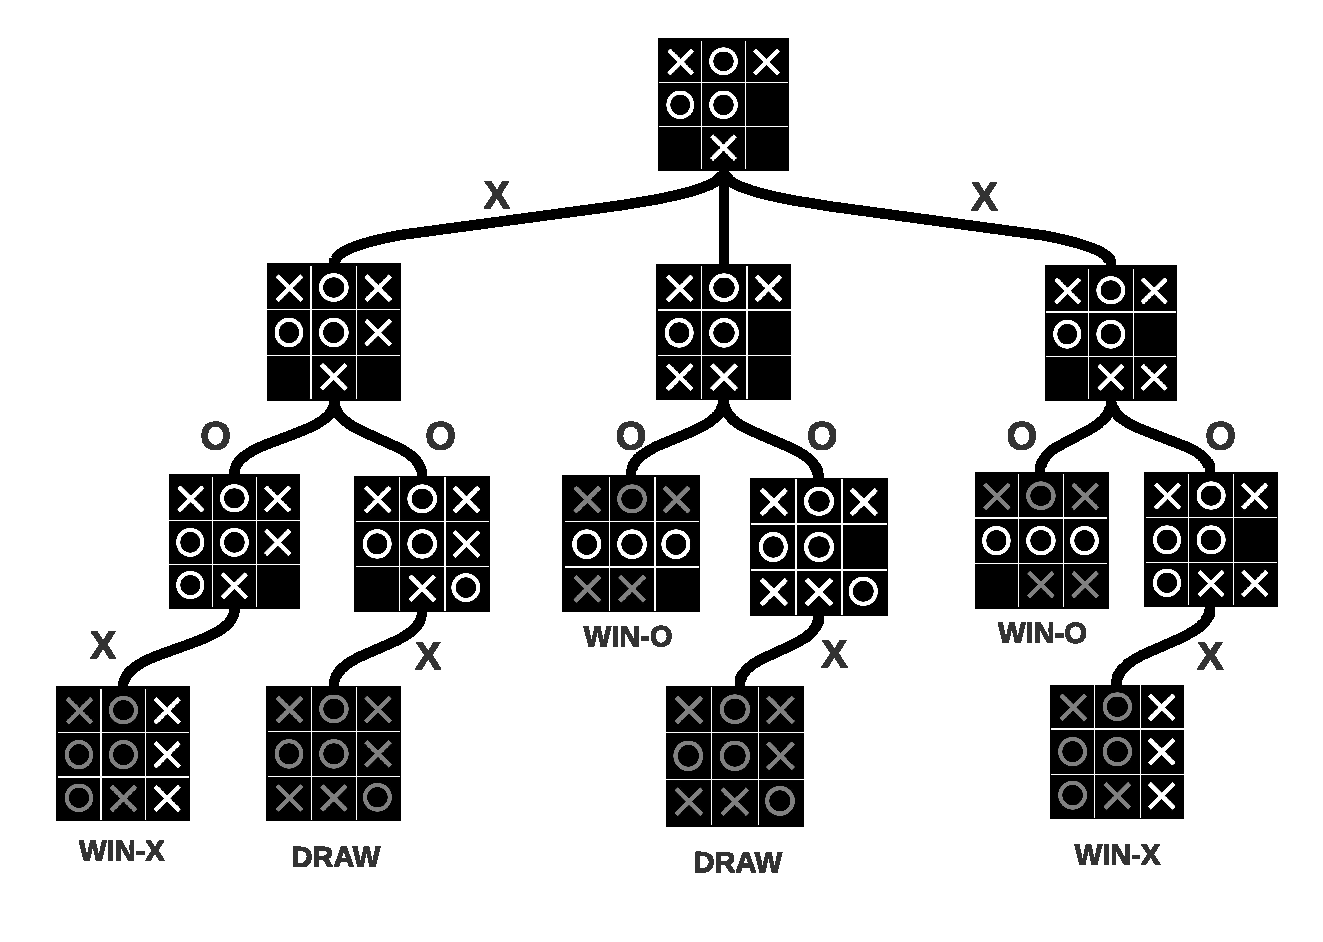
\includegraphics[width=2.5in]{graph.pdf}
\caption{Game tree of Naughts and Crosses}
\label{fig_te}
\end{figure}

\subsection{Discussion of the solution}
Now that we have a clear understanding of state and transitions, lets discuss how to make a powerful agent that never looses the game. 

What if we have a agent which can peep into the future and judge which next state is best for it. This same concept is used in many game
playing programs like deep blue. The program just on the knowledge of the current state will iterate upto some depth $d$ in the game tree
and will try to choose that state which will maximize its chances of winning.

The minimax algorithm is complete in the sense that it finds the optimal solution, and if the game is optimal and someone is playing against the computer then, the computer
will never lose. But minimax has its own disadvantages, the major being the size of the state space. $\alpha-\beta$ pruning decreases the state space of the search as it
doesn't explore the nodes which have no effect on the output of the parent node in the game tree. The code of both the algorithms can be found \href{https://github.com/sid-tiw/AI-codes/blob/main/codes/min\_max\_improved.cpp}{here}.

\subsection {Complexity of the Alpha-Beta pruning}

In the best case of the Alpha-Beta pruning, if the effective branching factor is $b$, then the time required can be written as:
\[T(m) = T(m - 1) + (b - 1) \times T(m - 2) + O(1)\]
Where m is the height of the tree.\\
The characteristic equation for the recurrence relation given above:
\[x^2 - x - (b - 1) = 0\]
\[\implies x = \frac{1 \pm \sqrt{4 \times b - 3}}{2} = \pm O(b^{\frac{1}{2}})\]

So, the solution of this recurrence relation is given by (under the assumption that $b$ is greater than $1$):
\[T(m) = a \times O(b^{\frac{1}{2}})^{m} - b \times O(b^{\frac{1}{2}})^{m}\]
\[\implies T(m) = C \times O(b^{\frac{m}{2}}) = O(b^{\frac{m}{2}})\]


\begin{thebibliography}{9}
\bibitem{Travelling Salesman Problem}
Travelling Salesman Problem
\\\texttt{https://en.wikipedia.org/wiki/Travelling\_salesman\_problem}

\bibitem{ai} 
Stuart J. Russell and Peter Norvig. 2003.
\\\textit{Artificial Intelligence: A Modern Approach (2nd. ed.).}
Pearson Education.

\bibitem{test_case} 
Travelling Salesman Test Cases,
\\\texttt{http://www.math.uwaterloo.ca/tsp/vlsi/index.html\#XQF131}
\end{thebibliography}


\end{document}
